\documentclass[main]{subfiles}
\begin{document}

\section*{Lecture 14 // Oct 8 // Lifting to $\mathbb{Z}$-grading and the Filtered Chain Complex}
\addcontentsline{toc}{section}{Lecture 14 -- Lifting to Z-grading and the Filtered Chain Complex}

\begin{recall}
We defined the irreducible Instanton Chain Complex (ICC) $C(Y)$, which is a $\mathbb{Z}/8$ graded complex based at the reducible $\Theta$. The chain complex acts strangely at $\Theta$: the grading drops by $5$ for flows passing through it, so there's an issue with broken flowlines and $\partial^2$ isn't $0$.

We can get a chain complex with the reducible solutions by encoding the behavior at $\Theta$ into two maps.
\[
D_1 : C_1 \to \mathbb{F}, \text{ which encodes flows into } \Theta,
\]
\[
D_2 : \mathbb{F} \to C_{(-4)}, \text{ which encodes flows out of } \Theta.
\]
From these we can define two chain complexes for which $\partial^2=0$ by either forgetting flows into/out of $\Theta$:
\[
\overline{C} = C\oplus \mathbb{F}_0, \qquad \overline{\partial} = \partial + D_1,
\]
\[
\underline{C} = C\oplus \mathbb{F}_{(-3)}, \qquad \underline{\partial} = \partial + D_2.
\]
\end{recall}

\begin{question}
Why do we care about the reducible(s)?
\end{question}
\noindent\textit{Answer.} The cobordism maps usually come from the $D_1, D_2$ maps.

\subsection*{$\mathbb{Z}$-Lifted version of IFH}

We can lift the CS functional to be $\mathbb{R}$-valued (instead of $\mathbb{Z}$) by choosing a lift of $\mc{B}^\ast$ to the universal cover, $\widetilde{\mc{B}}^\ast$,
\[
\pi_1(\mc{B}^\ast) \cong \mathbb{Z}, \qquad \pi_1(\widetilde{\mc{B}}^\ast) = 1.
\]
Recall that $\pi_1(\mc{B}^\ast)\cong \mathbb{Z}$ since we are quotienting the space of connections, which is contractible, by $\mc{G}$, which has $\mathbb{Z}$-many path components, one in each degree. To get $\widetilde{\mc{B}}^\ast$, we must instead quotient by a subgroup of $\mc{G}$ which is $\mathbb{Z}$-times smaller, i.e., choosing one path component as a ``basepoint.'' The most obvious one to choose is the degree $0$ one.

\begin{definition}
The based gauge group is the subgroup $\mc{G}_0 \leq \mc{G}$ of degree zero gauge transformations
\[
\mc{G}_0 := \{g\in \mc{G} \mid \deg(g^{-1}) = 0\}.
\]
\end{definition}

By construction, $\pi_0(\mc{G}_0)=1$. Like before, we define the configuration spaces $\widetilde{\mc{B}}$ and $\widetilde{\mc{B}}^\ast$ by
\[
\widetilde{\mc{B}} = \mc{A}/\mc{G}_0, \qquad \widetilde{\mc{B}}^\ast = \mc{A}^{\mathrm{irred}}/\mc{G}_0.
\]
Note that $\widetilde{\mc{B}}^\ast$ is a $\mathbb{Z}:1$ cover of $\mc{B}^\ast$, so the Chern-Simons functional $\CS : \mc{B}^\ast \to \mathbb{R}/\mathbb{Z}$ lifts to a $\mathbb{R}$-valued map $\widetilde{\CS} : \widetilde{\mc{B}}^\ast\to \mathbb{R}$. Repeating the IFH construction, we obtain a $\mathbb{Z}$-graded complex over $\mathbb{F}[y^{\pm 1}]$, where $y$ is in degree $8$ and multiplying by $y$ encodes switching between lifts, so increases the value of the Chern-Simons functional by one.

\begin{center}
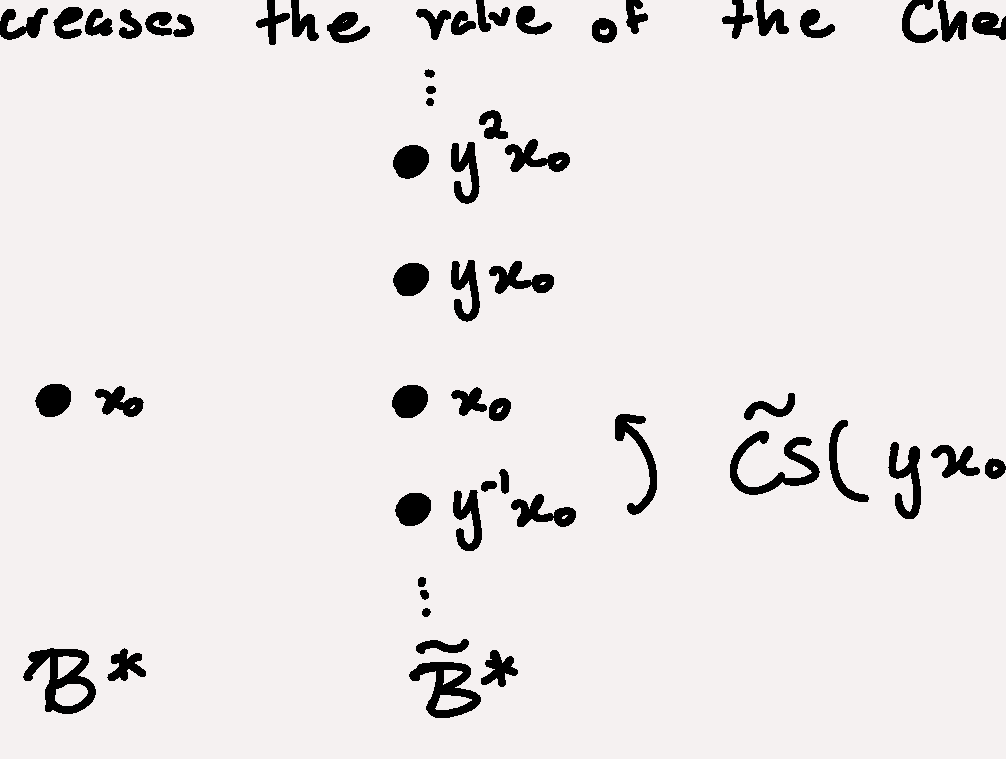
\includegraphics[width=0.45\linewidth]{figures/fig_lec14_tower_basic.png}
\end{center}
\[
\widetilde{\CS}(y\cdot x_0) = \widetilde{\CS}(x_0) + 1.
\]

We will also refer to the $\mathbb{Z}$-lifted version as $C(Y)$.
\[
\overline{C} = C\oplus \mathbb{F}[y^{\pm 1}]_{(0)}, \qquad \underline{C} = C\oplus \mathbb{F}[y^{\pm 1}]_{(-3)}.
\]

By trivializing the bundle, we get a connection for which $\widetilde{\CS}$ vanishes; we take this to be the lift of $\Theta$.

This filtration also descends to one on $\underline{C}$ and $\overline{C}$.

\begin{definition}
A filtered chain map $f : C_1\to C_2$ is a chain map which is non-increasing with respect to the filtration, i.e., $f(C_1^s)\subseteq C_2^s\ \forall s$.
\end{definition}

\begin{definition}
A filtered chain homotopy $H$ between filtered chain maps $f$ and $g$ is a chain homotopy for which $H(C_1^s)\subset C_2^s\ \forall s$. If $H$ exists for $f,g$, $f$ and $g$ are filtered chain homotopic.
\end{definition}

We claim that the filtered homotopy equivalence class (FHEC) of $C$ is an invariant of $Y^3$. To show this, we ask: what must we keep track of? What auxiliary data was used in our definition of $C(Y)$?

Well, the first thing we had to do for any bundle stuff was choosing a metric on $Y$. The critical points of $\CS(Y)$ don't depend on $g$: the point is that they're inherently topological, e.g., counting $\SU(2)$ representations of $\pi_1$. However, the differential does depend on $g$, since to even define a gradient-like vector field, we need a metric. Moreover, the definition uses the Hodge star! $\grad_A\CS = \ast_g F_A$.

So strictly speaking, the complex does depend on $g$ a priori. Thus we must check that changing $g$ doesn't change the FHEC.

There is a second thing. If CS doesn't have discrete critical points, we must perturb the CS functional to get discrete critical points. So far, we've brushed this fact under the rug; it's actually super annoying to deal with.

A random perturbation of CS functional (or even a general Morse function) will certainly change the value of CS at critical points. So we have no reason to think that any perturbation should play well with the CS filtration.

In reality, our definition of the IFC is incorrect. It's actually defined as a ``limiting object.'' The idea is that we can find an arbitrarily small sequence of perturbations $\{\pi_i\}_{i=1}^\infty$ for which $\widetilde{\CS}$ has discrete critical points. For each perturbation, we get a filtered complex $C^{\pi_i}(Y)$. If we do this with enough regularity, as $\|\pi_i\|\to 0$, these complexes converge to some limiting object which we define to be $C(Y)$:
\[
C^{\pi_i}(Y) \xrightarrow{\|\pi_i\|\to 0} C(Y).
\]

However, there are many cases for which a perturbation is not needed, in which case the definition is true as given. For example, the Brieskorn homology spheres $\Sigma(p,q,r)$ with three singular fibres have discrete critical points without a perturbation. Conceptually, we'll discuss the complex as if no perturbation is needed.

\subsection*{The Chern-Simons Filtration}

\begin{definition}
A $\mathbb{R}$-valued filtration on $C$ is a collection of subcomplexes $\{C_s\}_{s\in\mathbb{R}}$ such that
\begin{enumerate}
\item $C_r \subseteq C_s$ for $r\leq s$,
\item $\displaystyle\bigcup_s C_s = C$.
\end{enumerate}
\end{definition}

Given a filtered complex, we can get filtered subquotients $C^{[r,s]} = C^s/C^r$ for each pair $r\leq s$. Note that $[r,s]$ actually means $(r,s]$, so the generators $x\in C^{[r,s]}$ are the generators $x\in C$ with Chern-Simons value $r < \widetilde{\CS}(x) \leq s$.

Observe that $\widetilde{\CS}$ gives $C$ the structure of a filtered complex. For each generator (critical point), we can look at the value of the (perturbed) CS-functional at each $x$.

Diagrammatically, the filtration looks like the following. The values of CS for each generator are written in blue, and the complex is arranged vertically by $\mathbb{Z}$-grading.

\begin{center}
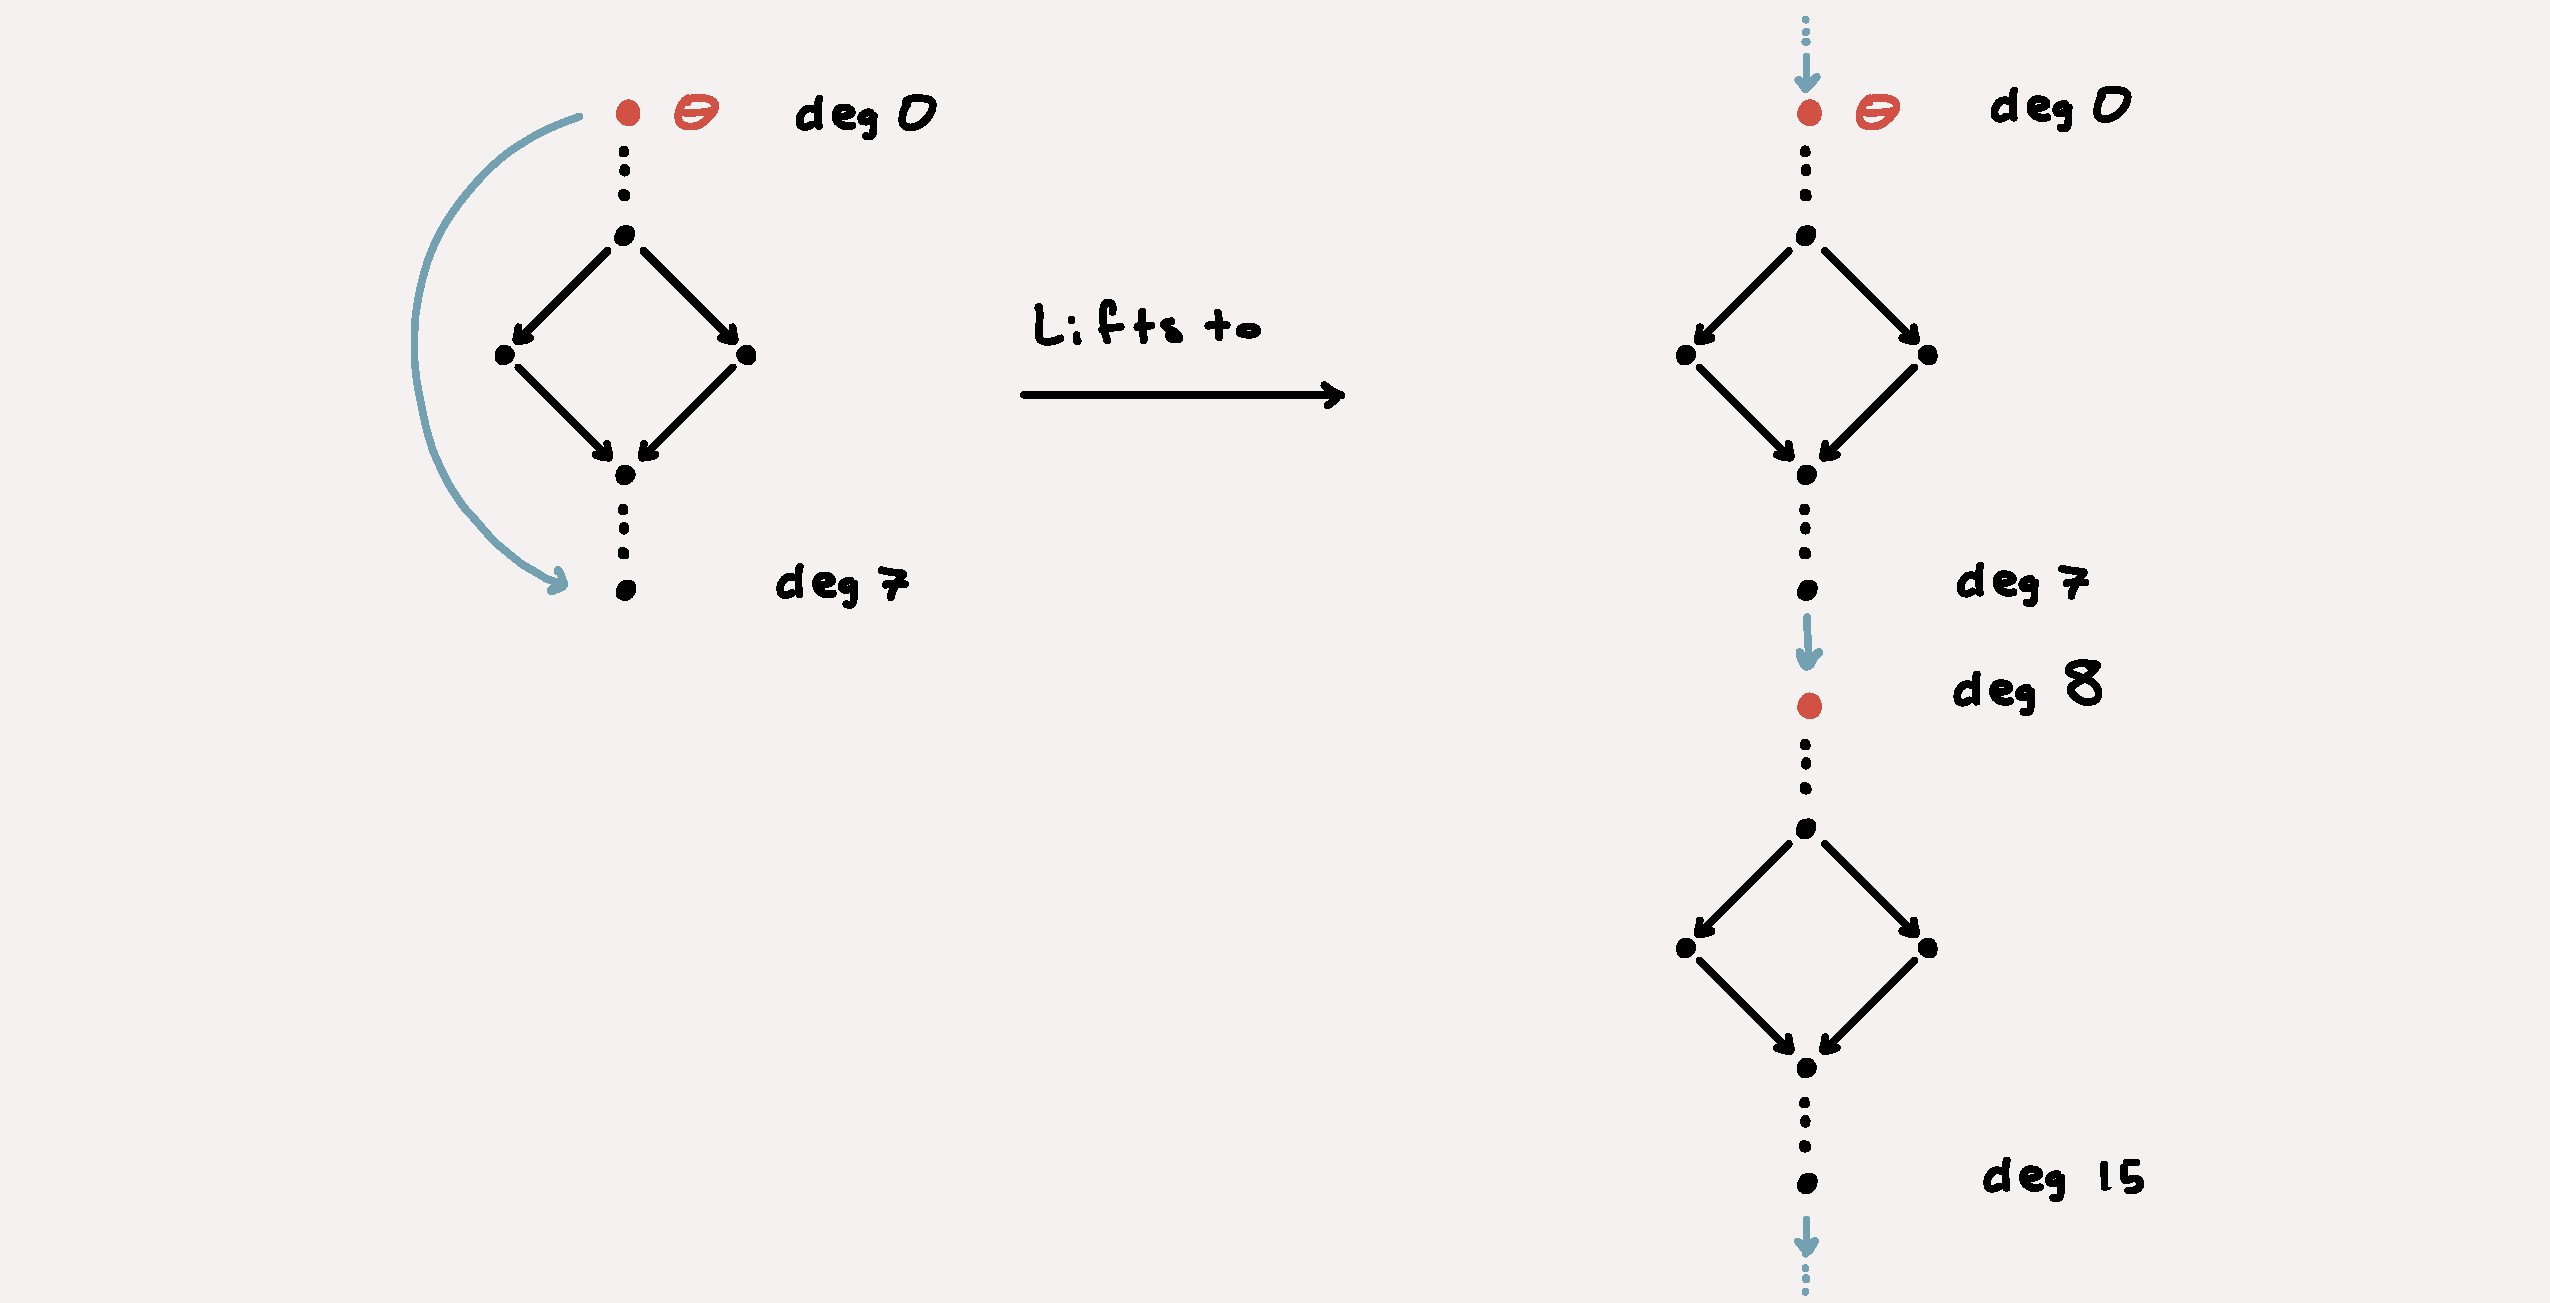
\includegraphics[width=0.9\linewidth]{figures/fig_lec14_lift_diamond.png}
\end{center}

\begin{center}
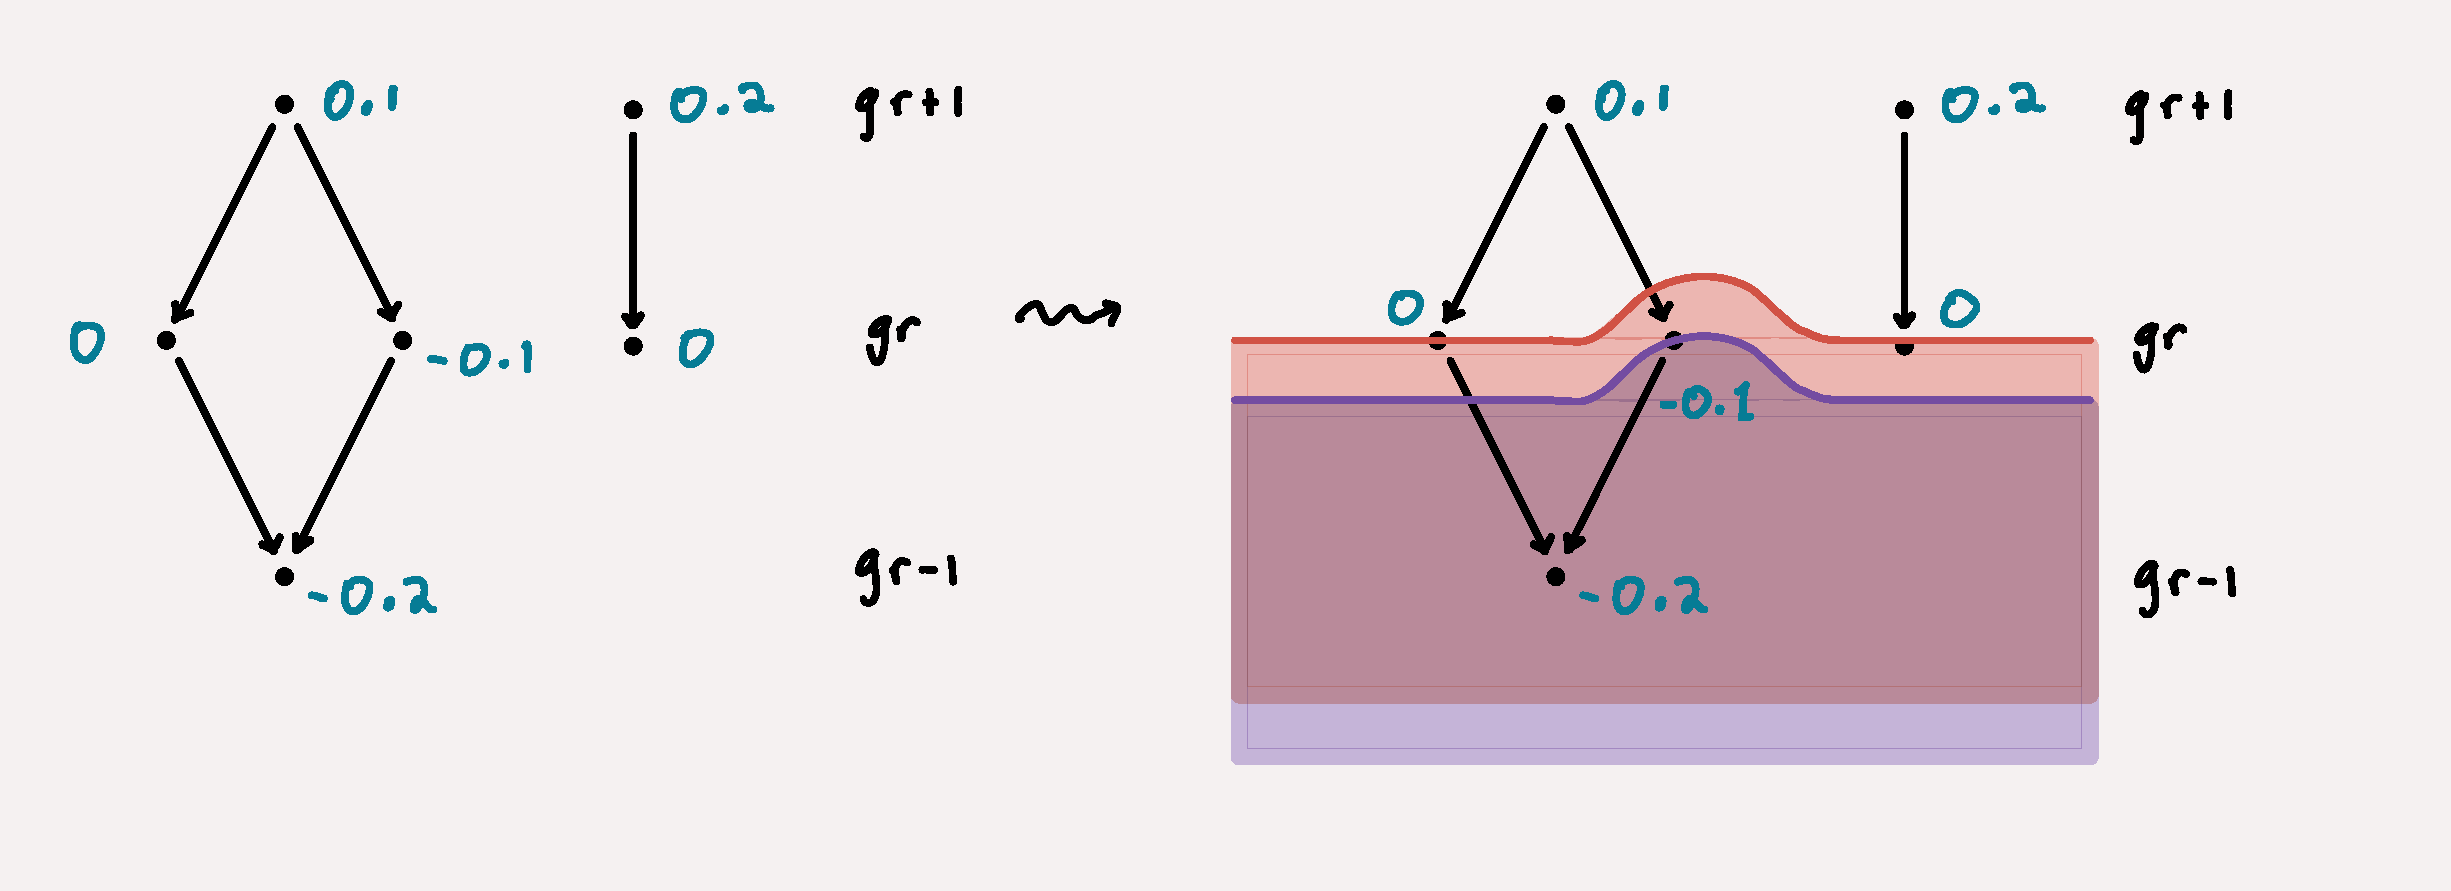
\includegraphics[width=0.9\linewidth]{figures/fig_lec14_filtration_vertical.png}
\end{center}

If this complex was instead arranged vertically by Chern-Simons value, the filtration would look like horizontal lines:

\begin{center}
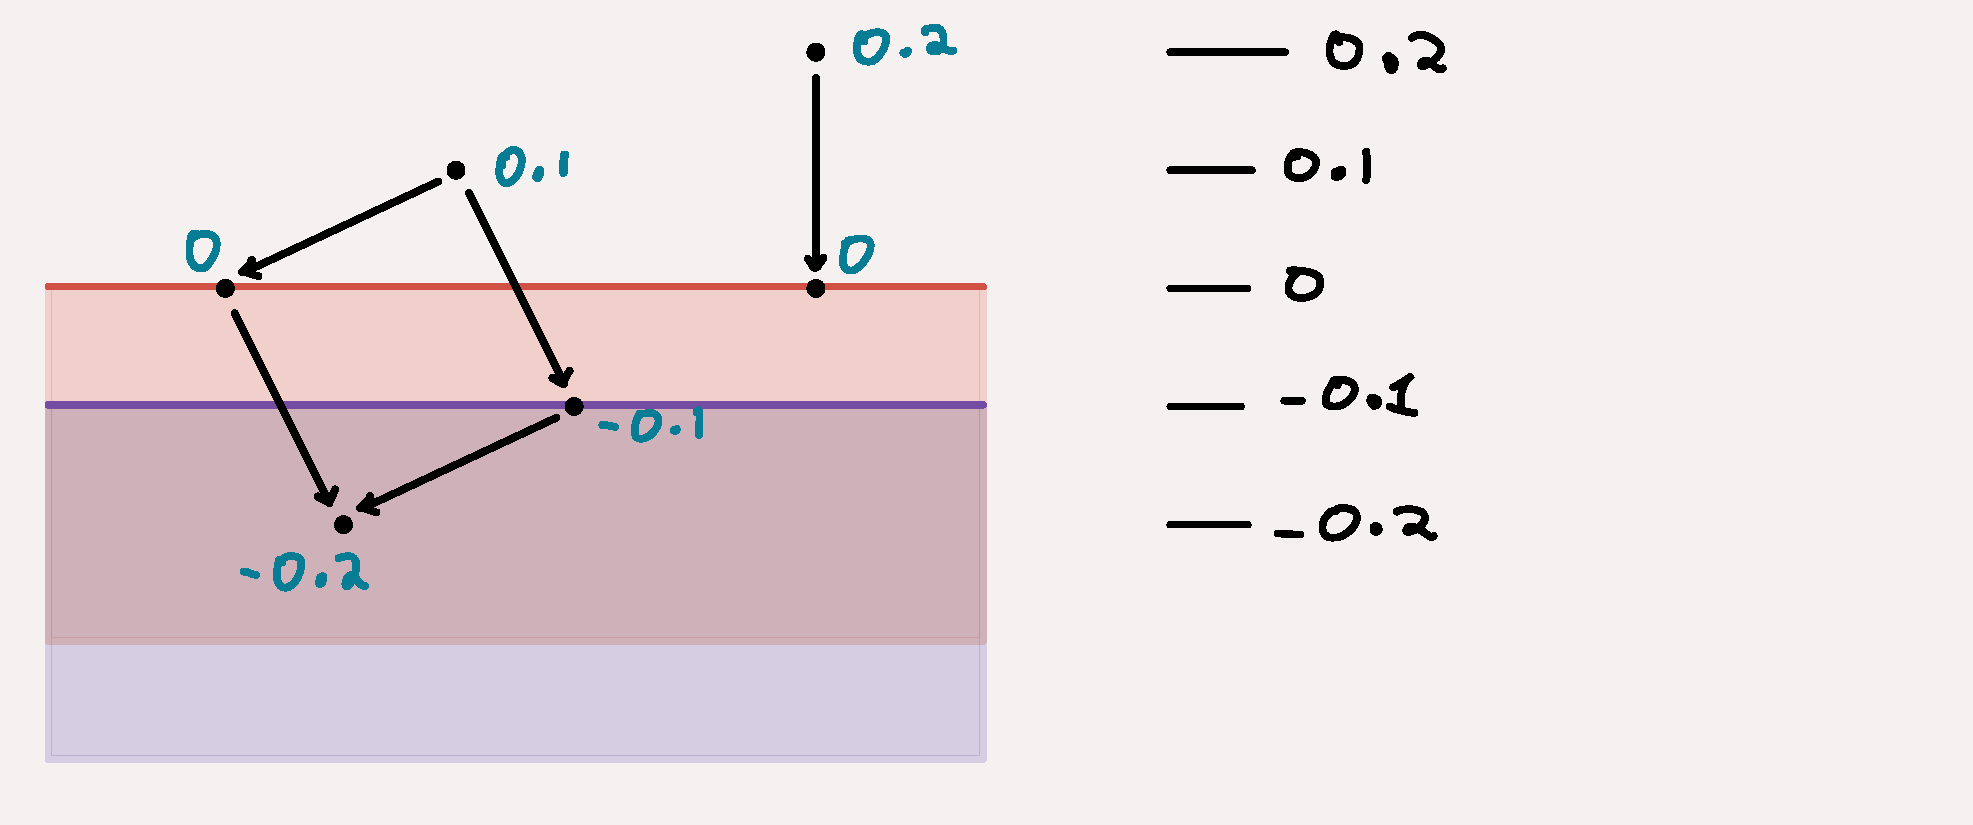
\includegraphics[width=0.75\linewidth]{figures/fig_lec14_filtration_horizontal.png}
\end{center}

\begin{remark}
The $\mathbb{Z}$-grading is independent from the CS value, but they both go down under the differential.
\end{remark}

\begin{remark}
If $\mc{B}^\ast$ has nontrivial $\pi_1$, then the grading shift for flows which use this $\pi_1$ is larger than one, since the expected dimension for the flowline is higher. Lifting to $\widetilde{\mc{B}}^\ast$ ``unwinds'' this $\pi_1$, so gradings always drop by $1$.
\end{remark}

\subsection*{Cobordism Maps}

If you've seen Floer theory before, you'll have heard of the so-called TQFT structure, e.g., ``bordisms induce maps.'' This is formalized as follows.

\begin{definition}
A Floer homology theory $F$ is said to have the structure of a TQFT if, for $W$ a cobordism from $Y_1$ to $Y_2$, there is a cobordism map $F_W : C(Y_1)\to C(Y_2)$.
\end{definition}

In our setting, let $W$ be a negative-definite cobordism with $b_1(W)=0$. From $W$, we construct the ``cylindrical end manifold'' $W^\ast$ by attaching $Y_1\times(-\infty,0]$ and $-Y_2\times[0,\infty)$ to their respective ends.

\begin{center}
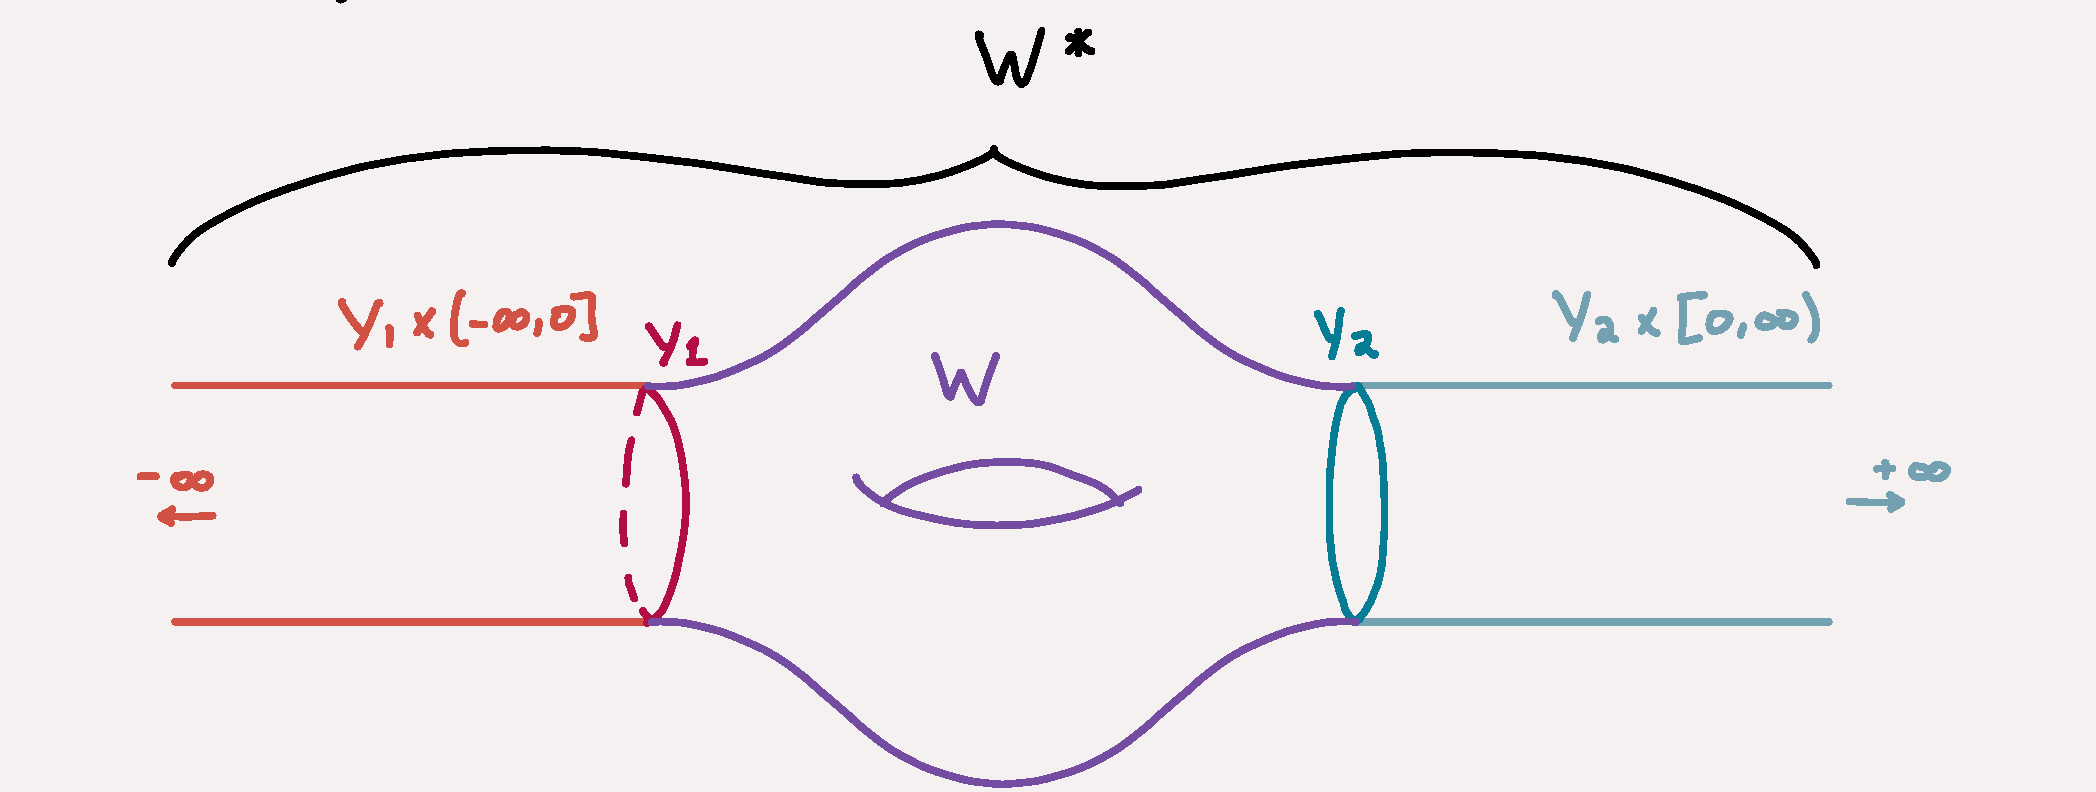
\includegraphics[width=0.9\linewidth]{figures/fig_lec14_cylindrical_end.png}
\end{center}

Consider the trivial bundle $W^\ast\times\mathbb{C}^2$. Given $x\in C(Y_1)$ and $y\in C(Y_2)$, look at ASD connections on $W^\ast$ which limit to $x$ and $y$ (on the left and right, respectively), modulo gauge transformations on $W^\ast$. As with $\partial$, the space of connections on $W^\ast$ modulo gauge on $W^\ast$ has many different topological components. We can think about this as follows.

On $Y_1$ and $Y_2$, $x$ and $y$ are really just representatives of gauge equivalence classes $[x_0]$ and $[y_0]$ of connections on $Y_1$ and $Y_2$.

If $g^\ast y_0 \in [y_0]$, then we also want to count connections limiting to $x_0$ and $g^\ast y_0$. As with before, we claim there is no gauge transformation on $W^\ast$ sending a connection from $x_0\to g^\ast y_0$ to one from $x_0\to y_0$. In particular, if $g$ is a gauge transformation on $W^\ast$, then $\deg(g|_{Y_1}) = \deg(g|_{Y_2})$.

\begin{exercise}
Prove the claim.
\end{exercise}

This shows that there are $\mathbb{Z}$-many topological classes of connections interpolating between $x_0$ and $y_0$, determined by the difference of degree $\deg(g_1)-\deg(g_2)$ for gauge transformations $g_1$ on $Y_1$ and $g_2$ on $Y_2$. Diagrammatically, this can be seen by quotienting by a vertical $\mathbb{Z}$-shift:

\begin{center}
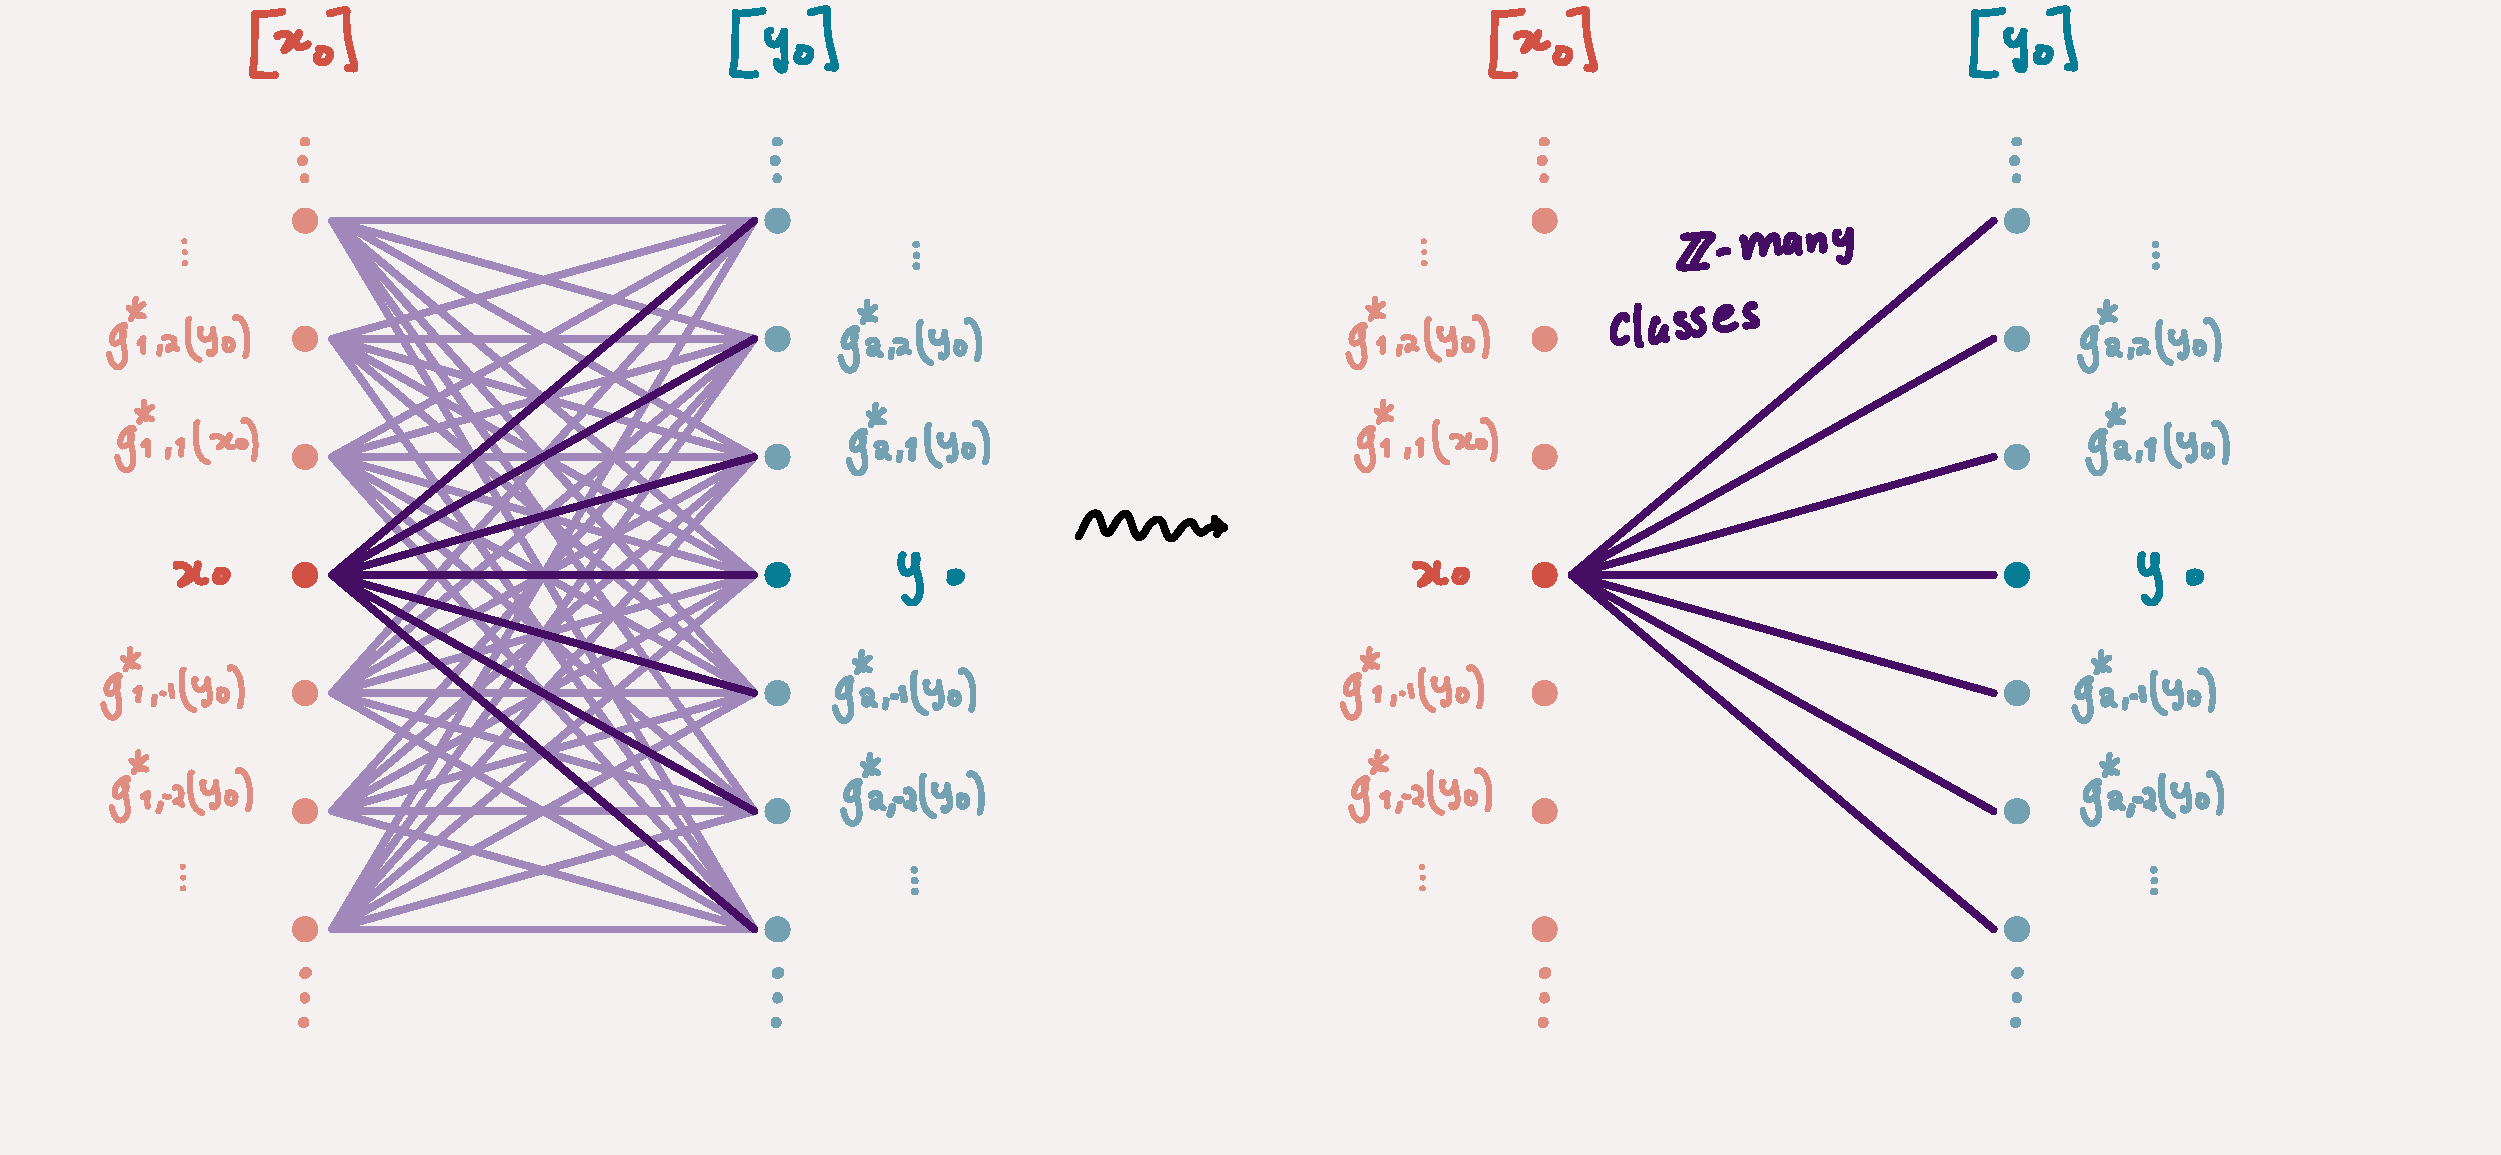
\includegraphics[width=0.9\linewidth]{figures/fig_lec14_many_classes.png}
\end{center}

\end{document}
